\chapter{Resultat}

\section{Partikelrörelse i celler}

\subsection{Isometri}

%\subsection{Anisometri} Från givna data kunde en viss tendens till anisometri\todo{anisotropi?} anas då partiklarna tenderade att röra sig längs med vissa riktningar. En minstakvadratanpassning för en rät linje gjordes för att kunna transformera de givna $x$- och $y$-koordinaterna till tangent- och normalkoordinater relativt den anpassade linjen för varje partikel. För dessa nya koordinater beräknades en tidskorrelation vilket visas i \figref{fig:Korr_tn} för både aktiva celler och celler i dvala.

%Tillfällig bild, kan förbättras
%Bör definitivt ändras till eps eller pdf.
%\begin{figure}
%    \centering
%    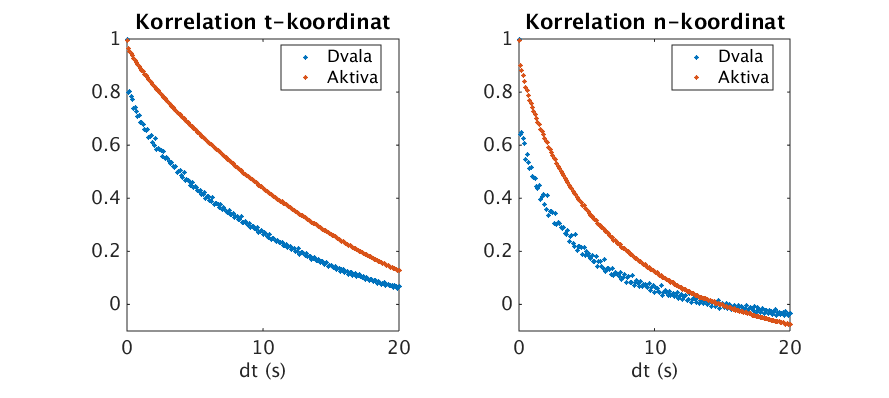
\includegraphics[width=.8\textwidth]{Korrelation_tnkoordinat.png}
%    \caption{Korrelation i tangent- och normal-koordinaterna för aktiva celler och celler i dvala. I båda fall sjunker korrelationen initialt snabbare för cellerna i dvala. Korrelationen tycks även bestå längre i tangentialkoordinaten än normalkoordinaten vilket tyder på att det finns en föredragen väg.}
%    \label{fig:Korr_tn}
%\end{figure}

\subsection{Avvikelse från brownsk rörelse}
%Har vi exempel på avvikelse från teorin kan dessa läggas under seprata underrubriker här

\paragraph{MSD}
Utifrån teorin kring Brownsk rörelse kan vissa förutsägelser göras för partiklar som strikt följer denna typ av rörelse. Bland annat räknades det fram i avsnitt~\ref{sec:brown} att mean square displacement (MSD) för en sådan partikel skulle öka linjärt med tiden, se ekvation \todo{}\eqref{eq:MSD_brown}. Utifrån givna data för arbetet har ett potenssamband kunnat anpassas med en exponent som är skilld från och betydligt lägre än 1. Detta tyder på att partikeln inte utför en ren brownsk rörelse utan genomgår en så kallad subdiffusion, karakteriserat att partikelns MSD beror av tiden via ett potenssamband med exponent mindre än 1 men större än 0.

\begin{figure}
    \centering
    \includegraphics[width=.8\textwidth]{MSD_lilla_delta.png}
    \caption{Från filen MSD.m}
    \label{fig:MSD_ld}
\end{figure}

Vidare finns det minst två sätt att beräkna partiklarnas MSD. För stationära processer, dvs processer som inte explicit beror på när i tiden de inleds, kan man skapa ett medelvärde mellan alla möjliga mätpunkter separerade med givet tidsintervall så som beskrivet i ekvation ...
\todo{Kanske bör vi lägga till ett stycke om hur egenskaperna beräknas utifrån diskret data}
Genom att jämföra resultatet från denna typ av beräkning med att istället bara ta medelvärdet mellan alla partiklars kvadrerade radiella avvikelse från startpunkten vid given tid från start kan man avgöra om processen är stationär.
\todo{Bild för jämförelse mellan lilla och stora delta}
Båda dessa beräkningar har utförts för given data och exponentens värde i sambandet mellan MSD och tid skiljer sig/överensstämmer för lite för att någon tydlig slutsats hurvida processen är stationär eller ej ska kunna dras. \todo{Eller?}

\begin{figure}
    \centering
    \includegraphics[width=.8\textwidth]{MSD_stora_delta.png}
    \caption{Från filen storleksberoende.m}
    \label{fig:MSD_sd}
\end{figure}


%%%%%%%%%%%%%%%%%%%%%%%%%%%%%%Strängar%%%%%%%%%%%%%%%%%%%%%%%%%%%%%%


\section{Strängars rörelse i vätskor}




%Bara en liten kodsnutt som behövs när man kompilerar lokalt
%%% Local Variables: 
%%% mode: latex
%%% TeX-master: "main.tex"
%%% End: 
